\documentclass[12pt,a4paper]{article}
% \usepackage[subpreambles=true]{standalone}
\usepackage[a4paper]{geometry}
\usepackage[utf8]{inputenc}
\usepackage[T1]{fontenc}
\usepackage[light]{CormorantGaramond}
\usepackage{import}

\linespread{1.25}

\usepackage{amsmath, amssymb, amsfonts, amsthm, mathtools}
\newcommand{\R}{\mathbb{R}}
\newcommand{\Z}{\mathbb{Z}}
\newcommand{\argmin}{\arg\!\min} % AlfC
\DeclareMathOperator{\tr}{tr}
\newcommand{\irchi}[2]{\raisebox{\depth}{$#1\chi$}}
\newcommand{\rchi}{{\mathpalette\irchi\relax}}
\usepackage{algorithm}
\usepackage{algpseudocode}
\usepackage{float}

\usepackage{microtype} %improves the spacing between words and letters

\usepackage{lipsum}
\usepackage{threeparttable}
\usepackage{tabularx}
\usepackage{multirow}
\usepackage{booktabs}
\newcommand{\tabitem}{~~\llap{\textbullet}~~}
\usepackage{graphicx}
\graphicspath{ {./pics/} {./eps/}}
\usepackage{epsfig}
\usepackage{epstopdf}
\usepackage{diagbox}
\usepackage{sidecap}

\sidecaptionvpos{figure}{c}

%%%%%%%%%%%%%%%%%%%%%%%%%%%%%%%%%%%%%%%%%%%%%%%%%%
%% COLOR DEFINITIONS
%%%%%%%%%%%%%%%%%%%%%%%%%%%%%%%%%%%%%%%%%%%%%%%%%%
\usepackage[dvipsnames]{xcolor} % Enabling mixing colors and color's call by 'svgnames'
%%%%%%%%%%%%%%%%%%%%%%%%%%%%%%%%%%%%%%%%%%%%%%%%%%
\definecolor{MyColor1}{rgb}{0.2,0.4,0.6} %mix personal color
\definecolor{MyColor2}{HTML}{A30073}
\definecolor{MyColor3}{HTML}{A3008F}
\definecolor{LightCoral}{HTML}{FF7287}
\newcommand{\textb}{\color{Black} \usefont{OT1}{lmss}{m}{n}}
\newcommand{\blue}{\color{MyColor1} \usefont{OT1}{lmss}{m}{n}}
\newcommand{\blueb}{\color{MyColor1} \usefont{OT1}{lmss}{b}{n}}
\newcommand{\red}{\color{LightCoral} \usefont{OT1}{lmss}{m}{n}}
\newcommand{\green}{\color{Turquoise} \usefont{OT1}{lmss}{m}{n}}
%%%%%%%%%%%%%%%%%%%%%%%%%%%%%%%%%%%%%%%%%%%%%%%%%%

%%%%%%%%%%%%%%%%%%%%%%%%%%%%%%%%%%%%%%%%%%%%%%%%%%
%% FONTS AND COLORS
%%%%%%%%%%%%%%%%%%%%%%%%%%%%%%%%%%%%%%%%%%%%%%%%%%
%    SECTIONS
%%%%%%%%%%%%%%%%%%%%%%%%%%%%%%%%%%%%%%%%%%%%%%%%%%
\usepackage{titlesec}
\usepackage{sectsty}
%%%%%%%%%%%%%%%%%%%%%%%%
%set section/subsections HEADINGS font and color
\newcommand*{\myfont}{\fontfamily{cmr}\selectfont}
\chapterfont{\myfont \color{MyColor1}}
\sectionfont{\myfont \color{MyColor1}}
\subsectionfont{\myfont\color{MyColor1}}  % sets colour of sections

%set section enumerator to arabic number (see footnotes markings alternatives)
% \renewcommand\thechapter{\arabic{chapter}.} %define chapters numbering
% \renewcommand\thesection{\arabic{section}.} %define sections numbering
% \renewcommand\thesubsection{\thesection\arabic{subsection}} %subsec.num.

%%%%%%%%%%%%%%%%%%%%%%%%%%%%%%%%%%%%%%%%%%%%%%%%%%
%		CAPTIONS
%%%%%%%%%%%%%%%%%%%%%%%%%%%%%%%%%%%%%%%%%%%%%%%%%%
\usepackage{caption}
\usepackage{subcaption}
%%%%%%%%%%%%%%%%%%%%%%%%
\graphicspath{{./figures/}} %Setting the graphicspath
% \graphicspath{{./figures/G&D/}} %Setting the graphicspath
% \captionsetup[figure]{labelfont={color=Turquoise}}

%%%%%%%%%%%%%%%%%%%%%%%%%%%%%%%%%%%%%%%%%%%%%%%%%%
%		!!!EQUATION (ARRAY) --> USING ALIGN INSTEAD
%%%%%%%%%%%%%%%%%%%%%%%%%%%%%%%%%%%%%%%%%%%%%%%%%%
%using amsmath package to redefine eq. numeration (1.1, 1.2, ...)
%%%%%%%%%%%%%%%%%%%%%%%%
\renewcommand{\theequation}{\thesection\arabic{equation}}

%set box background to grey in align environment
\usepackage{etoolbox}% http://ctan.org/pkg/etoolbox
\makeatletter
\patchcmd{\@Aboxed}{\boxed{#1#2}}{\colorbox{black!15}{$#1#2$}}{}{}%
\patchcmd{\@boxed}{\boxed{#1#2}}{\colorbox{black!15}{$#1#2$}}{}{}%
\makeatother
%%%%%%%%%%%%%%%%%%%%%%%%%%%%%%%%%%%%%%%%%%%%%%%%%%

\makeatletter
\let\reftagform@=\tagform@
\def\tagform@#1{\maketag@@@{(\ignorespaces\textcolor{red}{#1}\unskip\@@italiccorr)}}
\renewcommand{\eqref}[1]{\textup{\reftagform@{\ref{#1}}}}
\makeatother
\usepackage{hyperref}
\hypersetup{colorlinks = true, linkcolor  = black}

%% LISTS CONFIGURATION %%
\usepackage{enumitem}
\setlist[enumerate,1]{start=1}
\renewcommand{\labelenumii}{\theenumii}
\renewcommand{\theenumii}{\theenumi.\arabic{enumii}.}
\newcommand{\cri}[1]{\textcolor{MyColor2}{\textbf{(Cri says: #1)}}}

%%%%%%%%%%%%%%%%%%%%%%%%%%%%%%%%%%%%%%%%%%%%%%%%%%
%% abbreviations:
%%%%%%%%%%%%%%%%%%%%%%%%%%%%%%%%%%%%%%%%%%%%%%%%%%
\usepackage[acronym]{glossaries}
\newacronym{pca}{PCA}{Principal Component Analysis}
\newacronym{svd}{SVD}{Singular Value Decomposition}
\newacronym{gsp}{GSP}{Graph Signal Processing}
\newacronym{omp}{OMP}{Orthogonal Matching Pursuit}

%%%%%%%%%%%%%%%%%%%%%%%%%%%%%%%%%%%%%%%%%%%%%%%%%%
%% PREPARE TITLE
%%%%%%%%%%%%%%%%%%%%%%%%%%%%%%%%%%%%%%%%%%%%%%%%%%
\title{\blue Homework Network Science course - Part2}
\author{Cristina Gava\\%
Matr 1153449}
\date{\today}
%%%%%%%%%%%%%%%%%%%%%%%%%%%%%%%%%%%%%%%%%%%%%%%%%%
%
% \usepackage{afterpage}
%
% \newcommand{\blankpage}{\null \thispagestyle{empty} \addtocounter{page}{-1} \newpage}

\begin{document}
\maketitle
In this second part of the work I focused on the behavior of the network related to the community detection and prediction and ranking of nodes and links.

\section*{Link prediction}
In the first part several link prediciton techniques has been applied, in order to see how the network responded: the methods used here are \textit{Common neighbour, Adamic Adar, Resource allocation, Katz} and \textit{Local Path}. First of all a certain amount of links has been removed from the network, in order to simulate a sort of temporal evolution of it and I then evaluated the performance of the algorithms. The removed edges have been:
\begin{itemize}
  \item The links related to the highest degree nodes;
  \item The links related to the lowest degree nodes;
  \item Some random links;
\end{itemize}
In \autoref{tab:lp} the results are displayed: here the focus was on the value of \textit{Precision factor} (out of all links, how many of them are predicted correctly), the \textit{Recall factor} (out of all actual links, how many of them are predicted correctly), the \textit{F-measure} (which helps to measure Precision and Recall at the same time using armonic mean and representing how much the two values are comparable) and finally the \textit{AUC measure} (which indicates how much the model examined is able to distinguishe between the classes, in this case the true new links and the false ones).

\begin{table}
\centering
\begin{tabular}{l|c|c|c|c}
  \toprule
  \multicolumn{5}{c}{\textbf{Highest degree node removal}}\\
  \midrule
  \diagbox{Methods}{Parameters} & Precision & Specificity & F-measure & AUC value\\
  \midrule
  Common neighbour & 0.9303 & 0.9348 & 0.9639 & 0.7172\\
  Adamic Adar & 0.9035 & 0.9120 & 0.9493 & 0.4061\\
  Resource Allocation & \red{0.0590} & \red{0.5152} & \red{0.1114} & \red{0.1204}\\
  Katz & 0.9705 & 0.9714 & 0.9850 & 0.8734\\
  Local Path & \green{0.9732} & \green{0.9739} & \green{0.9864} & \green{0.8003}\\
  \midrule
  \multicolumn{5}{c}{\textbf{Lowest degree node removal}}\\
  \midrule
  \diagbox{Methods}{Parameters} & Precision & Specificity & F-measure & AUC value\\
  \midrule
  Common neighbour & 0.9330 & 0.9372 & 0.9653 & 0.9477\\
  Adamic Adar & 0.9330 & 0.9372 & 0.9653 & 0.6708\\
  Resource Allocation & \red{0.9249} & \red{0.9302} & \red{0.9610} & \red{0.6700}\\
  Katz & \green{0.9732} &\green{0.9739} & \green{0.9864} & 0.9673\\
  Local Path & 0.9705 & 0.9714 & 0.9850 & \green{0.9732}\\
  \midrule
  \multicolumn{5}{c}{\textbf{Random degree node removal}}\\
  \midrule
  \diagbox{Methods}{Parameters} & Precision & Specificity & F-measure & AUC value\\
  \midrule
  Common neighbour & 0.9410 & 0.9443 & 0.9696 & \red{0.8242}\\
  Adamic Adar & 0.9276 & 0.9325 & 0.9624 & 0.8546\\
  Resource Allocation & \red{0.9223} & \red{0.9279} & \red{0.9596} & 0.8656\\
  Katz & \green{0.9732} & \green{0.9739} & \green{0.9864} & \green{0.9422}\\
  Local Path & \green{0.9732} & \green{0.9739} & \green{0.9864} & 0.9323\\
  \bottomrule
\end{tabular}
\caption{Comparison o the different link prediction algorithms wrt to three different types of removed links}
\label{tab:lp}
\end{table}
While the values of Precision, Specificity and F-measure are comparable in all the three cases and quiet good also, the more variability is present in the AUC value: it can be seen how Katz and Local Path methods always perform better than the other ones, while the Resource Allocation algorithm is always the one that performs poorly, compared to the others. If we then evaluate the AUC values with respect to the type of links removed, we can see an improvement in performance going from a lowest degree nodes link removal, to a highest one, passing through the random removal (in this case the function used was based on the generation of random values taken from a uniform distribution, so that the links were removed uniformly across the network). From these results we can conlude that in general the network behvaiour is predicted more precisely when it is composed by highly connected nodes.
\cite{repo}
\section*{Community detection}
For this part two approaches have been explored: in the first one a spectral clustering algorithm was employed, which took advantage of the Fiedler's eigenvetor (and so the minimum in the conductance values) to identify the two main communities of the network. The behaviour of the conductance is shown in \autoref{fig:cond}, where the minimum corresponds to the point over which is possible to perform the cut. The network so separated is shown in \autoref{fig:fiedler} and consists of $2$ communities of $68$ and $59$ elements respectively, with the minimum value for the conductance equal to $0.61863$.

\begin{figure}
\centering
\begin{minipage}{.47\textwidth}
  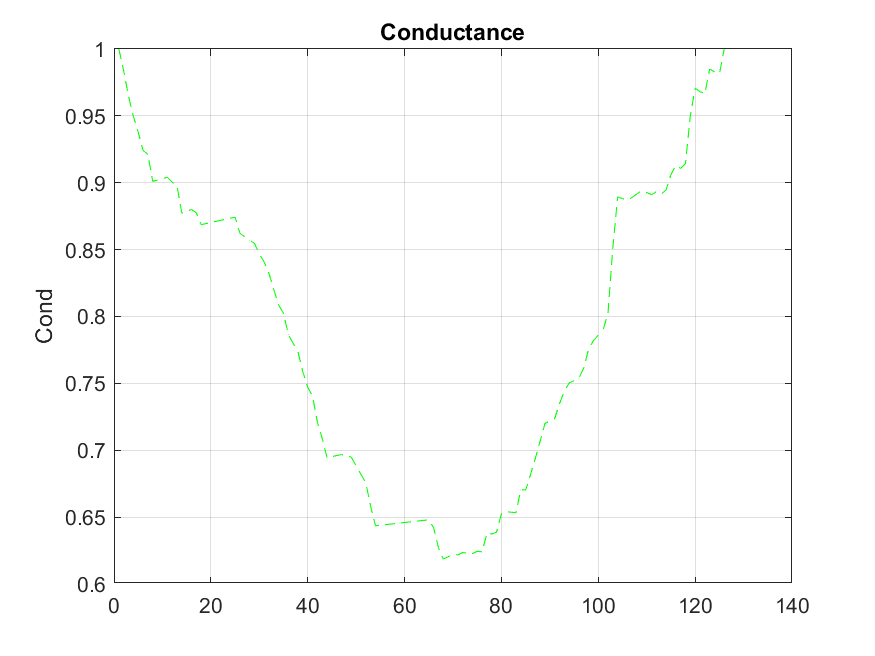
\includegraphics[width = \textwidth]{img/Conductance}
  \caption{Conductance trend}
  \label{fig:cond}
\end{minipage}
\begin{minipage}{.47\textwidth}
  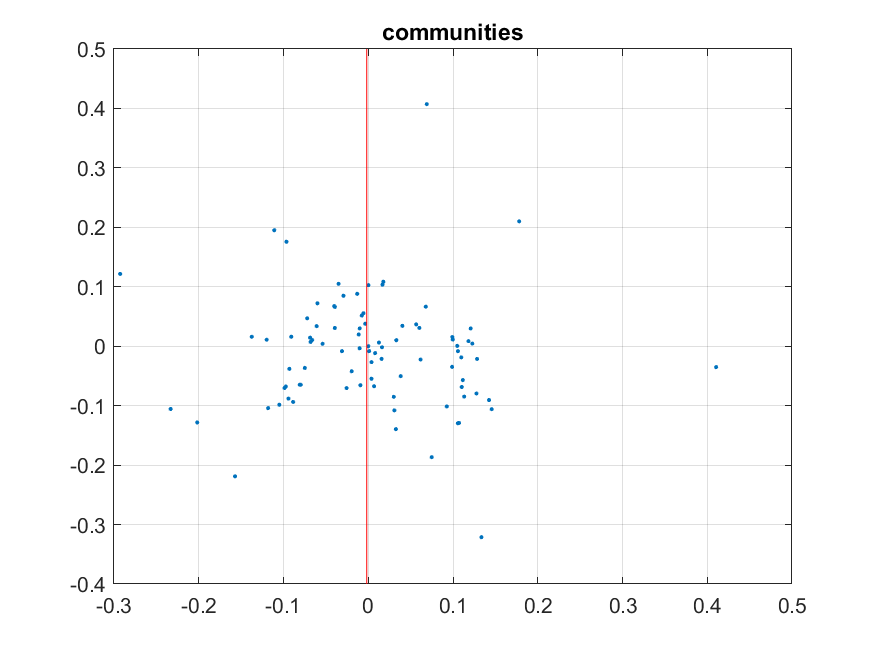
\includegraphics[width = \textwidth]{img/Communities}
  \caption{Communities separation}
  \label{fig:fiedler}
\end{minipage}
\end{figure}
The second approach used the PageRank-Nibble procedure, where the conductance value in this case was determined by the sweep over the nodes ordered according to the PageRank algorithm. In this case the communities found were definitely more unbalanced and the conductance value was quiet lower. The community separation is shwon in \autoref{fig:condNibble} and \autoref{fig:fiedlerNibble}, while \autoref{tab:cond} summarizes conductance and community measures. Precisely, in the table also the Cheeger's bound is listed, and from tht it can be observed how both of the clustering options found are suitable in this case, since both of them have values for conductance $<$ than that bound. In particular, the second approach has the lowest value of it, and this could indicate that the corresponding community separation is the best one.
\begin{figure}
\centering
\begin{minipage}{.47\textwidth}
  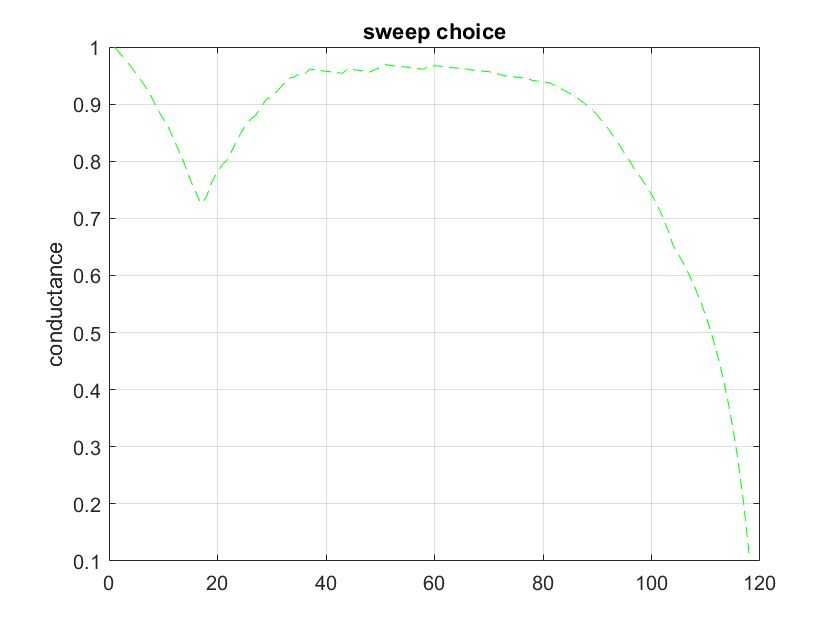
\includegraphics[width = \textwidth]{img/condNibble}
  \caption{Conductance trend}
  \label{fig:condNibble}
\end{minipage}
\begin{minipage}{.47\textwidth}
  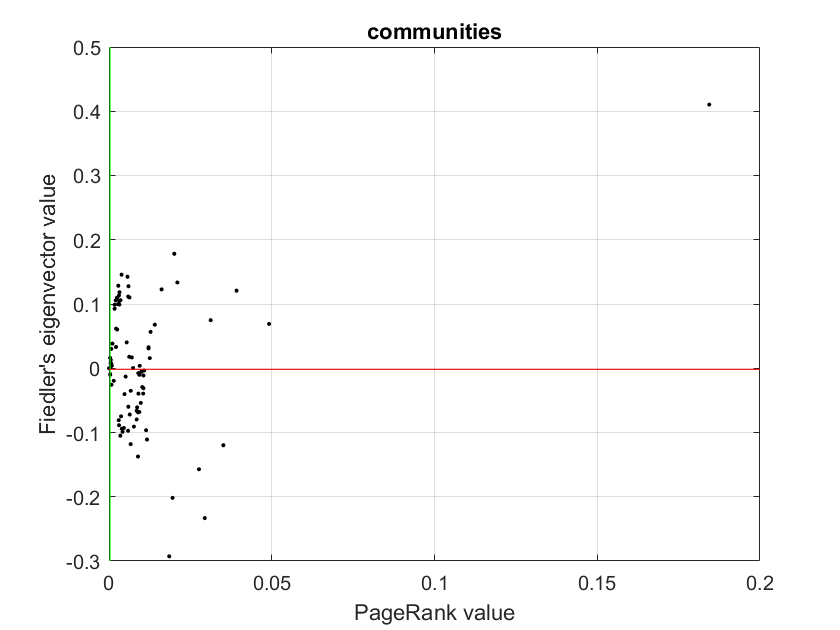
\includegraphics[width = \textwidth]{img/CommunitiesNibble}
  \caption{Communities separation}
  \label{fig:fiedlerNibble}
\end{minipage}
\end{figure}

\begin{table}
\centering
\begin{tabular}{cccc}
\toprule
                    & Minimum conductance & Community1 size & Community2 size\\
                    \midrule
Spectral clustering &   0.61863           & 68              & 59\\
PageRank-Nibble     &   0.11111           & 118             & 9\\
\midrule
Cheeger's bound     & \multicolumn{3}{c}{1.7493}\\
\bottomrule
\end{tabular}
  \caption{title}
  \label{tab:cond}
\end{table}

\section*{Ranking}
Another part of the owrk was dedicated to ranking, with a major look to the PageRank and the HITS algorithm respectively.
\subsection*{The PageRank algorithm}
First the work the PageRank approach has been investigated in details, in particular the linear system approach has been compared to the power iteration one and an estimate on the number of iterations required for the latter to converge has been found. \autoref{fig:PRconv}
\begin{SCfigure}
  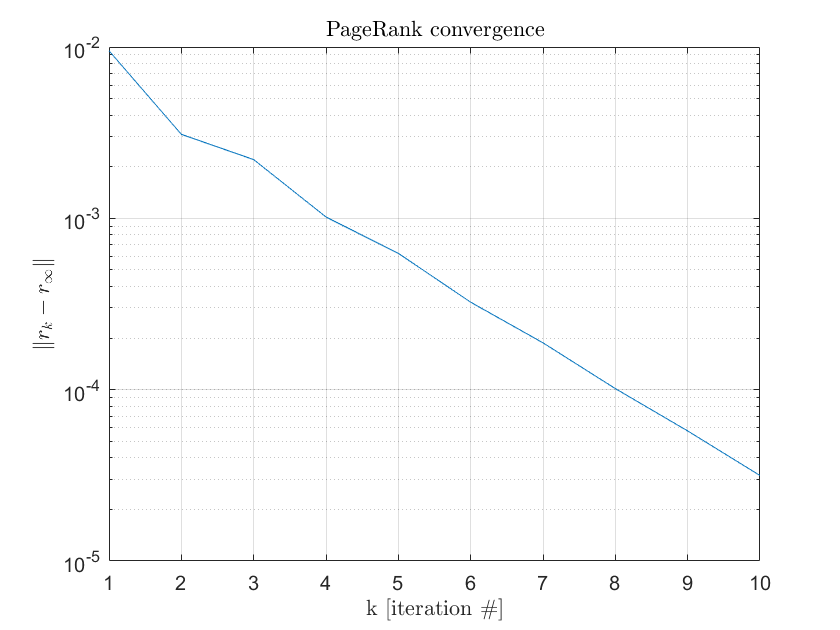
\includegraphics[width = .6\textwidth]{img/PageRank_Convergence}
  \caption{Convergence of the PageRank power iteration approach. From this it can be seen how the method converges quickly after a very small number of iterations}
  \label{fig:PRconv}
\end{SCfigure}
\begin{SCfigure}
  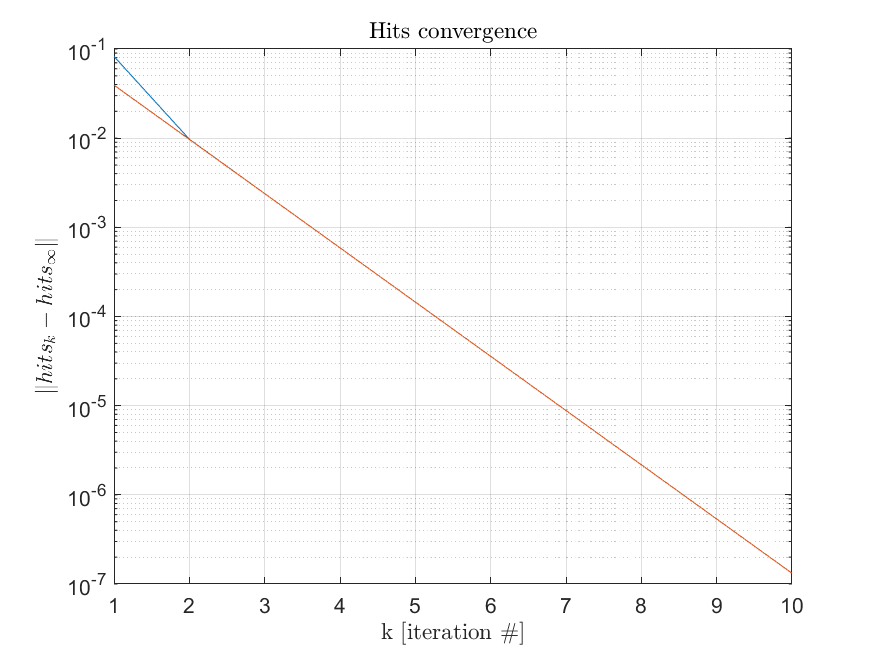
\includegraphics[width = .6\textwidth]{img/Convergence_hits}
  \caption{Convergence of the hits power iteration approach. This method is showed to converge approxhimately after 2 itertions}
  \label{fig:hitsConv}
\end{SCfigure}
\subsection*{HITS algorithm}
The other evaluation was made on the HITS approach, where the separation between hubs and authorities was not highlighted since the network we worked on is undirected. From \autoref{fig:hitsConv} it can be seen how also in this case the power iteration appraoch succesfully reaches convergence after a very limited number of iterations, $2$ in this precise case.
\subsection*{TrustRank algorithm}
Finally, particular attention have been put also on the implementation on a TrustRank version, in order to evaluate the robustness of the network to spamming behaviours. The damping factor has been se to $c = 0.85$ and the number of power iterations to $M_b = 20$. Following the indications in \cite{Garcia-molina2004}, the algorithm has been developed: the first part consisted of the description of the $\sigma-function$ and the \textit{Oracle function}, which were responsible, respectively, for the ordering of the nodes $wrt$ their seed score and for the expression
\begin{equation}
  \mathcal{O}(p) =
  \begin{cases}
    0 \quad \text{if $p$ is trustworthy}\\
    1 \quad \text{if $p$ is untrustworthy}
  \end{cases}
\end{equation}
that indicates whether a node can be considered good or not. The criteria selected to assign $0$ or $1$ to each seed was the belonging to one of the two communities found through spectral clustering. This supposition was based on the know idea that trustworthy nodes tend to connect/link to other trustworthy ones, while avoiding the spamming ones, in such way that the two categories can be seen as decently separated. The second part consisted in the actual implementation of the power iteration part, where we assumed a number $L$ of seeds supposed to be scanned manually and whose value actually comes from the oracle function, while the rest of the scores are evaluated and saved in the vector $trust$. The final scores are then checked, to see if they are above or beneath a certain threshold, and so, if their reliability has been estimated accordingly to the belonging to one of the two communities.

Finally, from the trust percentages found, conclusions on the goodness of the approach can be drawn: indeed, there is a percentage of trust $\%_{trust} = 41.51 \%$ (corresponding to the portion of nodes in the good community that are correctly estimated as good), and a percentage of distrust $\%_{distrust} = 75.68 \%$. While the former value is not very good (more that $50 \%$) of the good nodes are not seen as trustworthy, the latter is a good sign, since it shows that at least a great part of the bad nodes are recognized as such, concluding that the analyzed network is effectively scanned for "spamming" connections.
\begin{SCfigure}
  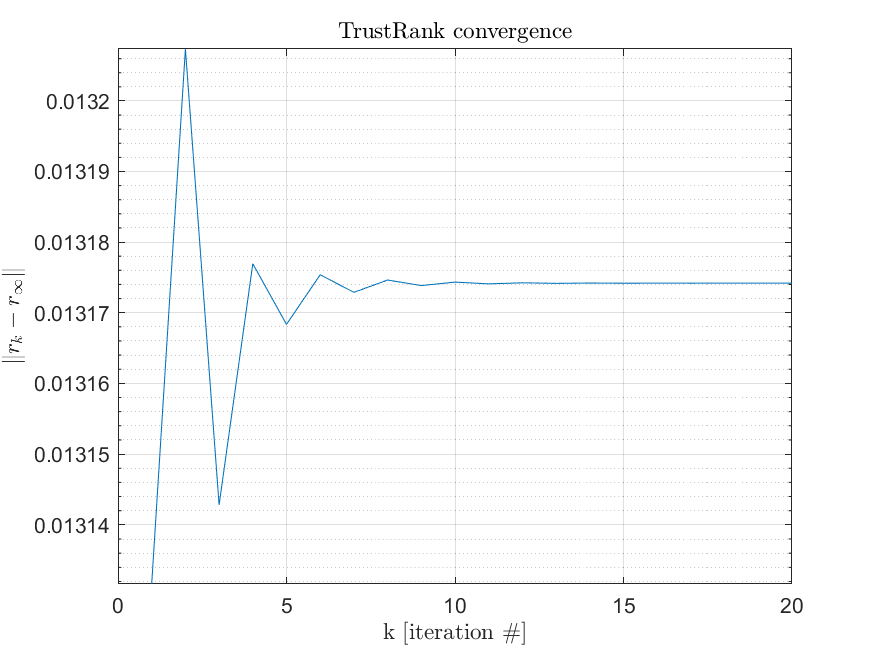
\includegraphics[width = .6\textwidth]{img/TrustRank_Convergence}
  \caption{Convergence of the TrustRank power iteration approach. Also here, it can be seen how the method converges rapidly in $< 10$ iterations.}
  \label{fig:trust}
\end{SCfigure}

\bibliographystyle{ieeetr}
\bibliography{BibHack}
\end{document}
